%\documentclass[prd,onecolumn,tightenlines,superscriptaddress,showpacs,nofootinbib,eqsecnum,amsfonts,amsmath]{revtex4}
\documentclass[preprint,onecolumn,,tightenlines,superscriptaddress,showpacs,nofootinbib,eqsecnum,amsfonts,amsmath]{revtex4}
\usepackage{bm,graphics,graphicx,epsfig,color,ulem,natbib, amssymb,amsmath}
%\usepackage{caption}
\usepackage{graphicx}
\usepackage{hyperref}
\usepackage[justification=raggedright,singlelinecheck=false,font=small,format=plain,labelfont=bf,up,textfont=normal,up]{caption}

\hypersetup{
    colorlinks=true,
    linkcolor=red,
    filecolor=red,
    urlcolor=red,
    citecolor=red,
}

%\allowdisplaybreaks

\def\be{\begin{equation}}
\def\ee{\end{equation}}
\def\ba{\begin{eqnarray}}
\def\ea{\end{eqnarray}}
\def\ud{\underline}
\def\lap{\lesssim}
\def\gap{\gtrsim}
\def\la{\langle}
\def\ra{\rangle}
\def\bse{\begin{subequations}}
\def\ese{\end{subequations}}
\def\bit{\begin{itemize}}
\def\eit{\end{itemize}}
\def\nn{\nonumber\\&}
\def\p{\partial}
\def\warning#1{\textcolor{red}{#1}}
\def\blue#1{\textcolor{blue}{#1}}
\def\red#1{\textcolor{red}{#1}}
\def\magenta#1{\textcolor{magenta}{\bf #1}}
\def\green#1{\textcolor{green}{#1}}

\def\ECM#1{\textcolor{green}{ECM: #1}}
\def\ARCH#1{\textcolor{black}{ARCH:#1}}
\def\ADAM#1{\textcolor{blue}{ADAM:#1}}
\def\HARIS#1{\textcolor{magenta}{HARIS:#1}}

%########################################################################################
\begin{document}
%%%%%%%%%%%%%%%%%%%%%%%%%%%%%%%%%%%%%%%%%%%%%%TITLE%%%%%%%%%%%%%%%%%%%%%%%%%%%%%%%%%%%%%%
\title{Harmonic analysis of the gravitational-wave waveform from precessing neutron star-black hole binary systems}
\author{K. Haris}\email{haris@iisertvm.ac.in}
\author{Kumar Atmjeet}\email{atmjeet@iisertvm.ac.in}

\author{Soham Mukherjee}\email{soham.m@iisertvm.ac.in}
\author{Archana Pai}\email{archana@iisertvm.ac.in}
\affiliation{Indian Institute of Science Education and Research Thiruvananthapuram, 
Computer Science Building, College of Engineering Campus, Trivandrum, Kerala, 
695016, India}
\author{\'Eric Chassande-Mottin}\email{ecm@apc.univ-paris7.fr}
\affiliation{APC, Univ. Paris Diderot, CNRS/IN2P3, CEA/Irfu, Obs de Paris, Sorbonne Paris Cit\'e, France}
%\captionsetup{justification=raggedright, singlelinecheck=false}
%%%%%%%%%%%%%%%%%%%%%%%%%%%%%%%%%%%%%%%%%%%%%%ABSTRACT%%%%%%%%%%%%%%%%%%%%%%%%%%%%%%%%%%%
\begin{abstract} 
  Compact binary systems of neutron stars and/or black holes undergoes
  precession when the spin of the primary object is not aligned with the orbital
  angular momentum. Precession results in the modulation of the emitted
  gravitational waveform which can be expressed in terms of a linear
  superposition of harmonics. Detection of individual harmonics from the
  advanced interferometric data would carry crucial astrophysical information
  about the precessing system. We evaluate the contribution to the
  signal-to-noise ratio of the various harmonics using the single-spin
  frequency-domain waveform model {\it SpinTaylorF2SingleSpin}. We show that the
  observation of the harmonics other than the $(2,2,2)$ mode provides
  direct evidence of precession.
  % Our study shows that mostly two of the harmonics are dominant in the \red{subspace of the
  % mass-spin parameter space for the binary with neutron star-black hole system
  % entire parameter space (nearly complementing each other) ADD: SOME QUANTITATIVE NUMBERS. 
  % ALSO ADD THE PARAMETER RECOVERY STATEMENT WHERE ETC AND WHAT BOUNDS?}
  % however, for high mass asymmetry and large spins some higher harmonics also do contribute to the waveform.
  % \ECM{Add one crisp summary sentence with quantitative statement. For
  % instance: We show that higher-order harmonics contribute significantly when
  % the spin is larger than XXX.}\ADAM{Check now if it looks appropriate}
\end{abstract}
%%%%%%%%%%%%%%%%%%%%%%%%%%%%%%%%%%%%%%%%%%%%%%%%%%%%%%%%%%%%%%%%%%%%%%%%%%%%%%%%%%%%%%%%%
\date{\today} \pacs{04.25.Nx, 04.30.-w, 97.60.Jd, 97.60.Lf} \maketitle
%%%%%%%%%%%%%%%%%%%%%%%%%%%%%%%%%%%%%%%%%%%%%%%%%%%%%%%%%%%%%%%%%%%%%%%%%%%%%%%%%%%%%%%%%

% \red{PAPER LAYOUT: - introduction/motivation  --	PARTIAL\\
% x context, GW150914, future LIGO/Virgo runs -- DONE \\
% x spinning waveforms have a reacher spectral contents including contribution from other modes than the usually dominating 2,2 mode \\
% x introduce spintaylorf2 and provide motivations for concentrating on this model --- DONE \\
% x objective: evidence the impact of spin on the relative amplitudes of the observed GW waveform \\
% x potential: simplification of search in certain areas of the parameter space; exhibit direct connection between the observed signal and important astro parameters in case such event is observed in future LV runs -- PARTIAL \\
% x outline of the paper \\ 
% - waveform overview -- NEEDS TO BE SHORTENED FURTHER, MORE REARRANGEMENT IS NEEDED \\
% x notations -- COORDINATE FIGURE NEEDS TO BE ADDED \\
% x introduce the necessary material about the waveform, harmonics decomposition --- NEED TO DISCUSS THE HARMONICS MORE (FIGURE MIGHT HELP) \\
% - analysis of dominating modes
% x description of the study \\
% x figures of merit: signal-to-noise ratio and overlap measurement \\
% x numerical simulations \\
% x results \\
% - discussion}
%=======================================================================================================%
%%%%%%%%%%%%%%%%%%%%%%%%%%%%%%%%%%%%%%%%% Introduction %%%%%%%%%%%%%%%%%%%%%%%%%%%%%%%%%%%%%%%%%%%%%%%%%%
%=======================================================================================================%

\section{Introduction}
\label{I}

% First detection of GW: BBH
A new era of astronomy has begun with the discovery binary black hole merger
events by the LIGO observatories
\cite{GW150914-DETECTION,GW151226-DETECTION}. These events reveal a yet
unobserved population of stellar-mass black holes with masses above $\sim 25$
solar masses \cite{GW150914-ASTRO}. More detections of such sources are expected
in the future as the sensitivity of Advanced LIGO \cite{GW150914-DETECTORS}
improves and as more detectors such as Virgo\cite{acernese15:_advan_virgo}, and
later KAGRA \cite{aso13:_kagra} and LIGO-India \cite{iyer11:_ligo_india} join
observations.

% We're interested in the NS-BH case
Future observations may also include other type of sources, and neutron
star-black hole (NS-BH) binary systems is one of the most promising. Those
systems are of particular interest as they may be connected to short-duration
gamma-ray bursts, see e.g. \cite{berger14:_short_durat_gamma_ray_burst}, thus
opening the possibility of multi-messenger observations where both
electromagnetic and gravitational-wave signals are detected from a single
astrophysical source.

% Importance of spin
The spin of the binary components carries important information. The measurement
of the spin may be decisive to understand how the binary formed. 

% Spins for NS-BH binaries
For NS-BH systems, the BH spin can, in principle, reach the relativistic limit.
On the contrary, the spin of the companion NS is much smaller. While isolated NS
can reach dimensionless spin $\sim 0.4$ in the case of PSRJ1748-2446ad
\cite{PSR2006}, the spin of NS in binary systems is likely much smaller
\cite{BROWN2012}. The fastest spinning pulsar in a double NS binary J0737–3039A
has a spin $\sim 0.05$ \cite{BURGAY2003}. For all practical purposes the spin of
NS can be neglected for NS-BH systems \cite{Lorimer:2008se}.

% Connection spin and precession
Arbitrarily oriented black-hole spin leads to the precession of binary orbit,
which causes the waveform modulation or equivalently the presence of
non-standard modes in the emitted gravitational-wave signal. The observation of
this modulation or of non-standard modes would thus evidence the presence of
precession, and thus provide information about the BH spin.

% Spins are measured by Bayesian estimates -- Need for a more direct clue
The source parameters (including spins) are estimated from the
gravitational-wave observations by fitting a waveform model using Bayesian
techniques \cite{Veitch:2014wba}. While such an approach has been successful in extracting
the astrophysical contents from the data, it is operated as a ``black box'' and
it does not exhibit explicitly the relation that exists between the waveform
features in the observations and the physics of the source.

% Objective of the paper
That is specifically the case for the relation between spin/precession and
waveform modulation/non-standard harmonics. This work is a study that
establishes quantitatively this relation through the harmonic analysis
of the {\it SpinTaylorF2SingleSpin} waveform model \cite{AS2014} which
is adapted to NS-BH binary systems.
 
In this work, we use the spin-harmonic structure of this waveform model to
identify the regions of mass-spin parameter space where different spin-harmonics of
{\it SpinTaylorF2SingleSpin} contribute. We then show how the harmonic contents
of the signal can be used to probe precession and in turn put bounds on spin
parameters.

% Paper outline
The paper is organized as follows. In Sec.~\ref{II}, we give an overview of the
{\it SpinTaylorF2SingleSpin} waveform model and compare it against its
time-domain variant \cite{Pan:2003qt,Buonanno:2009zt,Harry:2013tca}. We study
the signal-to-noise ratio using {\it SpinTaylorF2SingleSpin} in the mass-spin
parameter space. In Sec.~\ref{III}, we evaluate the relative contribution of the
in-built spin harmonics to the full waveform and identify the regions of the mass-spin 
parameter space where the main contributing modes dominate. Based on this, we further 
present an idea of probing the orientation parameter of the signal using these harmonics in Sec.~\ref{IV}.
Further we show how a bound on the BH spin can be obtained directly from the amplitude measurement 
of individual spin harmonics.

We follow the same notations of \cite{AS2014} in our study. We choose to work in
geometrical units, $G=c=1$.

% \ARCH{ADD SUMMARY -- 2 lines as what region of the space and what bound} 
%=======================================================================================================%
%%%%%%%%%%%%%%%%%%%%%%%%%%%%%%%%%%%%%%%%% Waveforms %%%%%%%%%%%%%%%%%%%%%%%%%%%%%%%%%%%%%%%%%%%%%%%%%%%%%
%=======================================================================================================%
\section{Gravitational-wave models for NS-BH systems}
\label{II}

We introduce the notations and waveform model for NS-BH inspiral system used for
this study. The BH quantities are labeled with the index $1$ {\it i.e.} mass
$m_1 \geq 3 M_\odot$ and dimensionless spin parameter $\chi_1 \sim
|S_1|/{m_1^2}$, with $0 \leq \chi_1 \leq 1$, and the NS quantities with index
$2$ such as mass $m_2 \approx 1.4 M_\odot$. We denote the total mass $M =
m_1+m_2$, the asymmetric mass ratio by $\eta = m_1m_2/(m_1+m_2)^2$ and the chirp
mass ${\cal M}_c=(m_1m_2)^{3/5}(m_1+m_2)^{-1/5}$. In case of precession, the
orbital angular momentum vector $\bf L$ and spin angular momentum vector $\bf
S_1$ precesses around the total angular momentum vector $\bf J = L+S_1$. This
precession primarily depends on the dimensionless spin $\chi_1$ and on the angle
between $\bf L$ and $\bf S_1$ measured by $\kappa = \bf {L} \cdot
{S}_1$. In this work we consider the case of \textit{simple precession}
where $\kappa$ is constant, ${\bf L}$ and ${\bf S_1}$ precess about ${\bf J}$
with the same angular speed and $\chi_1$ remains constant throughout the
precession cycle.
%=======================================================================================================%
%%%%%%%%%%%%%%%%%%%%%%%%%%%%%%%%%%%%%%%%% Overview waveforms %%%%%%%%%%%%%%%%%%%%%%%%%%%%%%%%%%%%%%%%%%%%
%=======================================================================================================%
\subsection{Overview about single-spin precessing waveforms}
\label{IIa}

The time-domain \textit{SpinTaylorT2} waveform model offers an alternative to
the two waveform families used in current compact binary searches namely, the
(time-domain) spin effective-one-body waveform tuned to numerical relativity
(SEOBNR) \cite{Taracchini:2013rva} and the (frequency domain)
inspiral-merger-ringdown phenomenological precession (IMRPP) waveform
\cite{Hannam:2013oca}. While the latter models provide complete waveforms (not
restricted to the inspiral phase but also covering the later merger and ringdown
phases), we do not require complete waveform for NS-BH as most of the SNR is in
the inspiral phase till BH mass $\sim 20 M_\odot$.\footnote{\green{For an aligned spin $(20-1.4)M_\odot$ system with $\chi_1=0.75$, the inspiral phase captures $\sim 90\%$ of total SNR.}}

Figure~\ref{fig:SPT2_waveform} shows typical gravitational-wave signals obtained
from \textit{SpinTaylorT2}. In Figure~\ref{fig:SPT2_waveform} (A), we consider a
non-spinning BH, $\chi_1=0$. In panels (B) and (C), the BH spin $\bf S_1$ is
aligned/anti-aligned to $\bf L$ for the same value for $\chi_1$. We note that
the waveform duration increases with $|\mathbf{J}|$.  The waveform is longer for
the aligned spin case (B), shorter for the non-spinning case (A) and even
shorter for the anti-aligned case (C). The rate of change of $\bf J$ depends on
the rate of change of the orbital angular momentum and is not affected by the
presence of spin. However since the total angular momentum varies with the
orientation of the spin vector. The length of the waveform shows this effect.
In Figure~\ref{fig:SPT2_waveform}(D), we show the inspiral waveform for an
arbitrarily oriented BH spin. The waveform is modulated because of the
precession of $\bf L$ and $\bf S_1$ about $\bf J$. The effect of waveform
amplitude and phase modulation is evident. In addition to the inspiral time
scale, the precession introduces a new time scale which is responsible for the
waveform modulation. The rate of precession also changes during the inspiral
phase which results into the variation in modulations over the inspiral phase.

\begin{figure}
 \centering
 %\captionsetup{justification=raggedright, singlelinecheck=false}
 \includegraphics[width=5in]{figures/waveform}
  \caption{SpinTaylorT2 time-domain waveforms for spinning and non-spinning NS-BH binary with 
 $m_1=14~M_{\odot}$ (BH) and $m_2=1.4~M_{\odot}$ (NS). Panel A: non-spinning BH with $\chi_1=0$. 
Panels B, C and D correspond to the cases with aligned spin ($S_{1z}=0.8$, i.e. $\chi_1=0.8$ and $\kappa=1$), 
anti-aligned spin ($S_{1z}=-0.8$, i.e. $\chi_1=0.8$ and $\kappa=-1$) 
and arbitrary spin orientation ($S_{1x}=S_{1y}=-0.7$, i.e. $\chi_1= 0.98$ and $\kappa=0$) respectively.}
\label{fig:SPT2_waveform}
\end{figure}
%=======================================================================================================%
%%%%%%%%%%%%%%%%%%%%%%%%%%%%%%%%%%%%%%%%% FD-Waveform %%%%%%%%%%%%%%%%%%%%%%%%%%%%%%%%%%%%%%%%%%%%%%%%%%%
%=======================================================================================================%
\subsection{Review of frequency-domain single-spin approximants}
\label{IIb}

The \textit{SpinTaylorF2SingleSpin} waveform model \cite{AS2014} results from
the stationary phase approximation of the Fourier transform of
\textit{SpinTaylorT2} waveform \cite{SPT21,SPT2} presented above. It provides a
convenient closed-form frequency-domain model for the inspiral phase of GW from
the NS-BH binary. As this is a generic, frequency-domain and analytical model
specially designed for the inspiral phase of the NS-BH systems, we choose to
work with this model to study the harmonics.

The {\it SpinTaylorF2SingleSpin} waveform is characterized by seven parameters:
the two mass parameters $m_1$ and $m_2$, the BH spin magnitude $\chi_1$ and
geometrical parameters including the angle $\kappa$ characterizing the
orientation of spin vector with respect to the angular momentum vector, the
orientation of $\bf J$ expressed by $\theta_J$ and $\psi_J$ with respect to the
line of sight and the azimuthal angle $\alpha_0$ of $\bf L$ in the inertial
frame aligned to the total angular momentum $\bf J$.

The observer's (inertial) frame is related to the source frame (co-rotating
frame attached to the binary) by three time-dependent Euler angles $\alpha,
\beta,$ and $\zeta$. The angle $\alpha$ is the precession angle of ${\bf L}$
about ${\bf J}$, $\beta$ is the opening angle of the precession cone and $\zeta$
is applied to minimize the co-ordinate changes associated with orbital plane
\cite{ACS1994}. The precession angle $\alpha$ changes over the precession time
scale associated to the modulation shown in Figure~\ref{fig:SPT2_waveform}, (D)
whereas $\beta$ varies over the time scale associated to the orbital decay
during the inspiral phase. Typically, the precession time scale is much smaller
than the inspiral time scale, and $\beta$ can be considered to remain constant
over several precession cycles. The assumption that the orbital phase is 
independent of $\alpha$ and $\zeta$, which implies that the precession-induced
phase varies much slowly than the orbital phase allows and justifies
the usage of stationary phase approximation used by authors of \cite{AS2014} to
obtain {\it SpinTaylorF2SingleSpin} waveform.

In the inertial frame the waveform is expressed in terms of the source amplitude $h^{\ell,m}$ as \cite{AS2014},
\begin{equation}
\label{h}
h_+ - i h_\times =e^{-2i \psi_J} \displaystyle \sum_{\ell,m',m} D_{m', m}^{(\ell)}(\alpha, \beta, \zeta) h^{\ell, m} \mathstrut_{-2} Y_{\ell, m'}(\theta_J,\phi) e^{-i m \Phi},
\end{equation}
where $D^{(\ell)}_{m', m}$ is the Wigner rotation matrix representation of SU(2) and $\Phi$ is the orbital phase. 

The expressions of the spin dependent harmonics $h^{\ell, m}$ are given in \cite{waveforms2009,waveforms2011}.

In the frequency-domain, the real part and $'+'$ polarization of the quadrupole
$(2,2)$ mode {\it i.e. $\ell=2$} in Eq.~(\ref{h}) can be expressed as
$\tilde{h}_+(f) = \sum_{m} \tilde{h}_{+m} (f)$ \cite{AS2014}, with
\begin{equation}
\label{hf}
\tilde{h}_{+m}(f) \simeq \left[A_{0}~f^{-7/6}~e^{i (\Psi(f) +\phi_0)}\right] \times \left[z_m~e^{i [m \alpha(f) -2\zeta(f)]}\right].
\end{equation}

The above equation explicitly separates in square brackets the {\it
  non-precessing} and {\it precessing} contributions to the mode.  The
non-precessing part involves the Fourier phase $\Psi(f)\equiv 2\pi f
t(f)-2\Phi(t(f))$, the initial phase $\phi_0$ (signal phase at the time of
arrival) and constant amplitude $A_{0}$ given below by
\begin{equation}
 A_{0}=\sqrt{\frac{5}{96\pi}} \frac{2\pi {\cal M}_c^2}{D} (\pi M )^{-7/6}
 \end{equation}
where $D$ is the source distance.

The precessing part contains the normalized amplitude function $z_m$ which 
when expressed in terms of the spin-weighted spherical harmonics reads
\begin{equation}\label{zm}
z_m(\theta_J, \psi_J, \beta(f)) = \frac{4\pi}{5} \, \mathstrut_{-2}Y_{2,m}(\beta(f), 0)
\left[  e^{-2i\psi_J} \;  \mathstrut_{-2}Y_{2,m}(\theta_J,0) 
+ e^{2i\psi_J}  \; \mathstrut_{-2} Y_{2,-m}(\theta_J,0) \right]\,.
\end{equation}

The precession-induced phase $m\alpha(f)-2\zeta(f)$ introduces the modulation in the waveform.
 
The expression for $\tilde{h}_{\times}(f)$ can be obtained by replacing $\psi_J \rightarrow \psi_J+ \pi/4$ in Eq.~(\ref{zm}). 
Note that the frequency dependence of $\Psi(f)$, $\alpha(f)$ and $\xi(f)$ appears in phase, whereas $\beta(f)$ contributes to the amplitude through $z_m$. 

When projected on the detector frame, the individual harmonics results in the following strain
\begin{equation}\label{hmf}
 \tilde{h}_m(f)=F_{+}~\tilde{h}_{+m}(f)+F_{\times}~\tilde{h}_{\times m}(f),
\end{equation}
where the antenna pattern $F_{+}$ and $F_{\times}$ depend upon the location of source in the sky. 
The GW signal $\tilde{h}(f)$ received by the detector is simply the sum of all those contributions.

%=======================================================================================================%
%%%%%%%%%%%%%%%%%%%%%%%%%%%%%%%%%%%%%%%%% Faithfulness %%%%%%%%%%%%%%%%%%%%%%%%%%%%%%%%%%%%%%%%%%%%%%%%%%
%=======================================================================================================%
\subsection{Faithfulness of {\it SpinTaylorF2SingleSpin}}
\label{IIc}

In this section, we assess the faithfulness of {\it SpinTaylorF2SingleSpin} waveform to its time variant {\it SpinTaylorT2}. We calculate the overlap between 
the {\it SpinTaylorF2SingleSpin} and {\it SpinTaylorT2}. The overlap between the two times series $a(t)$ and $b(t)$ is defined as
\begin{equation}\label{eq:overlap}
{{\cal{O}}_{ab}} \equiv \frac{(a | b)} {\sqrt{ (a | a) (b | b)}} \,,
\end{equation}
where the noise-weighted scalar product between $a(t)$ and $b(t)$ is obtained by
\begin{equation}\label{eq:inner}
(a | b) = 4 \mathrm{Re} \left[ \int_{f_l}^{f_h} df \; \frac{\tilde{a}(f) \tilde{b}^*(f)}{S_n(f)} \right] \,,
\end{equation}
where $\tilde{b}^*(f)$ denotes the complex conjugate of $\tilde{b}(f)$. The integral is evaluated over the frequency interval from $f_l$ = 30Hz to $f_h$ = 2 kHz which encompasses the observable 
frequency bandwidth. %\ECM{Give values for $f_l$ and $f_h$}\ADAM{Done}. 
$S_n(f)$ denotes the one-sided power spectral density of the detector noise. We use the \textit{zero-detuning, 
high power} advanced LIGO noise model \cite{aLIGOSensitivity}. The phase and time offsets between $a$ and $b$ are adjusted to maximize the overlap. This maximized overlap is termed as the {\it match}.

We compute the match between the {\it SpinTaylorF2SingleSpin} and the {\it SpinTaylorT2} waveforms for a population of $100\,000$ binaries with parameters randomly drawn 
from $m_1 \in [5, 50] M_\odot$, $\chi_1 \in (0, 1)$, $\kappa \in (-1, 1)$, $\theta_J \in (0, \pi)$, $\psi_J \in (0, 2 \pi)$ and $\alpha_0 \in (0, 2 \pi)$. The Figure~\ref{STF2_STT2_Match} 
shows the histogram for the match between {\it SpinTaylorF2SingleSpin} and {\it SpinTaylorT2} waveforms. For 80 \% of the case, the match is larger than 0.9. However, less than $10 \%$ 
has a match smaller than $0.8$.  Figure~\ref{STF2_STT2_Match} indicates that those cases are exclusively associated to binaries with $\kappa<-0.5$ \cite{AS2014}. When $\kappa > -0.5$
the {\it SpinTaylorF2SingleSpin} waveform is reliable and consistent with {\it SpinTaylorT2}. We therefore restrict the rest of our analyses to this region of the parameter space.

\begin{figure}
	\centering
	%\captionsetup{justification=raggedright, singlelinecheck=false}
	\includegraphics[width=0.5\linewidth]{figures/STF2_STT2Match_7}
	\caption{{\bf Faithfulness of {\it SpinTaylorF2SingleSpin :}} 
	Histograms of overlap between {\it SpinTaylorF2SingleSpin } waveform and {\it SpinTaylorT2}. Blue histogram is  for binaries with $\kappa \in (-1.,1.)$,   red curve 
	for  $\kappa \in (-0.5,1.)$ and green  for  $\kappa \in (-1.,0.5)$. A large fraction of samples with overlap $< 0.8$ is for $\kappa < -0.5$.
	The binaries are sampled with $m_1 \in [5. M_\odot, 50 M_\odot],~ \chi_1 \in (0.,1.),~ 
	\kappa \in (-1.1.),~\theta_J \in (0.,\pi), ~ \psi_J \in (0, 2 \pi),~\alpha_0 \in (0, 2 \pi)$.}
\label{STF2_STT2_Match}
\end{figure}
%=======================================================================================================%
%%%%%%%%%%%%%%%%%%%%%%%%%%%%%%%%%%%%%%%%% SNR STF2 %%%%%%%%%%%%%%%%%%%%%%%%%%%%%%%%%%%%%%%%%%%%%%%%%%%%%%
%=======================================================================================================%
\subsection{Signal-to-noise ratio \textit{vs} BH mass and spin}
\label{snr_section}

In this section, we study the variation of signal-to-noise ration (SNR) of {\it SpinTaylorF2SingleSpin} waveforms across the mass-spin parameter space. 
Figure~\ref{snr_plot} shows the SNR $\rho = (h|h)^{1/2}$ of the waveform $h$ as a function of the binary orientation $\theta_J$ and spin orientation $\kappa$ 
for different masses and spins. We consider three BH masses $m_1=2, 4$ and $18 M_\odot$ (or equivalently $\eta = 0.24, 0.13$ and $0.08$) and three spin amplitudes 
$\chi_1 = 0.2, 0.5, 0.8$. The source distance is taken as $D=400$~Mpc.

The near equal-mass binary with $m_1 = 2 M_{\odot}$ ($\eta = 0.24$) in the top row provides a typical SNR map for similar to non-precessing systems where the SNR is maximum (minimum) in the face-on or face-off (edge-on) configurations irrespective of the spin orientation. Similar conclusions can be drawn from the left column with low spin ($\chi_1=0.2$) and independently of the mass asymmetry. Note, however, that the SNR grows with the BH mass.

In the bottom right panel (large mass asymmetry, high spin), the SNR map transitions $\kappa$ value to the reverse pattern for negative $\kappa$, typical of precessing systems, where the SNR is maximum in the edge-on configuration, and minima for the face-on or face-off configurations. This depicts the precession effect due to the spin alignment with respect to the angular momentum vector. Needless to say this effect is prominent for high spins.

% The rest of the panels displays the same behaviour with a lower degree of intensity and a transition at a lower $\kappa$ value.

In summary, Figure~\ref{snr_plot} shows evidence that precession leads to observable consequences for asymmetric, highly-spinning systems. For $\kappa$ close to 1 (aligned spin), the emission pattern is similar to non-precessing systems (maximum SNR obtained for face-on or -off). For small $\kappa$ values (anti-aligned spin), the emission pattern is reversed (maximum SNR for edge-on). In the intermediate region, the SNR results from an interplay between $\kappa$ and $\theta_J$.

\begin{figure}[!hbt]
\centering
%\captionsetup{justification=raggedright, singlelinecheck=false}
{
\includegraphics[width=.5\linewidth, height=3.2in]{figures/SNR_by_SNR_max_color_1}
\hspace{.1cm}
\includegraphics[trim=-.2cm -1.4cm 0 .22cm, width=.2in,height=2.9in]{figures/colorbar_afmhot_r}
} 
\caption{\textbf{Signal-to-noise ratio for different BH masses and spins.} The figure has $3 \times 3$ panels, each shows the ratio of SNR to the 
maximum SNR ($SNR_{max}$) which corresponds to $\eta=.08$ and $\chi_1=0.8$. 
The colorbar is scaled by this $SNR_{max}=20.16$. Within each panel, the horizontal and vertical axes correspond to the spin orientation $\kappa$ and binary 
orientation $\theta_J$ respectively. From left to right BH spin $\chi_1 = 0.2, 0.5$ and $0.8$. From top 
to bottom the black hole mass $m_{1} = 2, 8$ and $14 M_{\odot}$, which corresponds to $\eta = 0.24, 0.13$ and $0.08$ respectively. 
}
\label{snr_plot}
\end{figure}
%=======================================================================================================%
%%%%%%%%%%%%%%%%%%%%%%%%%%%%%%%%%%%%%%%%% Harmonics %%%%%%%%%%%%%%%%%%%%%%%%%%%%%%%%%%%%%%%%%%%%%%%%%%%%%
%=======================================================================================================%
\section{Dominating spin harmonics}\label{III}

The {\it SpinTaylorF2SingleSpin} waveform model is can be expressed as a sum of
spin harmonics $h_m$ (often termed as sidebands), defined in Eq.~(\ref{hf}). In
this section, we study the contribution of the different spin harmonics to the
full waveform by computing their overlap ${\cal{O}}_{m}$ $\equiv (h | h_m) /
\sqrt{ (h | h) (h_m | h_m)} $ in different regions of mass-spin parameter space.
%=======================================================================================================%
%%%%%%%%%%%%%%%%%%%%%%%%%%%%%%%%%%%%%%%%% Overlaps %%%%%%%%%%%%%%%%%%%%%%%%%%%%%%%%%%%%%%%%%%%%%%%%%%%%%%
%=======================================================================================================%
\subsection{Overlap for $m=-2,\dots,2$}\label{IIIa}

Figure~\ref{FIG7} displays the cumulative distribution of ${\cal{O}}_{m}$ for $m=-2,\dots,2$ computed over a population of $100\,000$ binary systems with parameters in the following 
ranges $m_1 \in [3, 20] M_{\odot}$, $\chi_1 \in (0, 1)$, $\kappa \in (-0.5, 1.0)$ and $\theta_J \in(0, \pi)$. We keep the remaining two parameters $\alpha_0$ and $\psi_J$ equal to zero 
for this exercise. 

The overlap of the second mode ${\cal{O}}_2$ appears to be close to unity for a large fraction of the parameter space ($\sim 80\%$ of points above $0.8$), indicating that this mode 
is the dominant spin-harmonic amongst all for the large fraction of the parameter space. However, the ${\cal{O}}_0$ distribution shows that $\sim 10 \%$ of points have ${\cal{O}}_0$ overlap $> 0.6$. Also, for
$\sim 13\%$ of the points, spin mode
($2,2,1$) contributes with overlap between 0.4 to 0.6 (which
could be significant only for very high SNR {\it i.e.} nearby systems). In this parameter space, the ($2,2,-2$) and ($2,2,-1$)
modes do not contribute to the overlap. Henceforth, we focus on  ($2,2,2$) and ($2,2,0$)
spin modes in rest of the study.

\begin{figure}[!htbp]
\centering
%\captionsetup{justification=raggedright, singlelinecheck=false}
{
%\includegraphics[width=3.4in,height=2.7in,angle=0]{figures/PDF_new}
\includegraphics[width=.5\linewidth,height=2.7in,angle=0]{figures/CDF_new}
} 
\caption{Cumulative distribution for the overlaps ${\cal{O}}_{m}$ of ($2,2,m$)
  modes for $m=-2,\dots,2$ with the full waveform. The distribution shows the fraction of binaries
  with ${\cal O}_m$ smaller than a given value.}
\label{FIG7}
\end{figure}
%=======================================================================================================%
%%%%%%%%%%%%%%%%%%%%%%%%%%%%%%%%%%%%%%%%% Overlap Comparison %%%%%%%%%%%%%%%%%%%%%%%%%%%%%%%%%%%%%%%%%%%%
%=======================================================================================================%
\subsection{Contributions of $m=2$ and $m=0$ modes across the parameter space}
\label{IIIb}

Figure~\ref{modes} shows the variation of ${\cal{O}}_2$ and ${\cal{O}}_0$ with
respect to the spin-orbit alignment parameter $\kappa$ and binary orientation
$\theta_J$ for different spins and masses, similar to the SNR plots in
Figure~\ref{snr_plot}. The two maps of ${\cal{O}}_2$ and ${\cal{O}}_0$ exhibit
complementary feature which indicates that the total SNR is divided into these
two dominant modes.

The $(2,2,2)$ mode appears to dominate (${\cal O}_2$ close to one, ${\cal O}_0$
small) for the binaries identified earlier in Sec.~\ref{snr_section} with
near-equal mass (top row in Figure~\ref{modes}) and asymmetric binaries with
low-spin (left column) and when the spin is aligned to $\bf{L}$ ($\kappa$ close
to 1) independently of the mass ratio. The $(2,2,0)$ mode gains overlap when
spin or mass asymmetry increases especially near the edge-on region. This mode
dominates over $(2,2,2)$ for precessing binaries i.e., with asymmetric masses,
high BH spin. We should also mention here for such cases there is a leakage of
overlap in the ($2,2,1$) mode for near face-on (-off) cases and with
anti-aligned spin and angular momentum ($\kappa$ close to -0.5). However, we
restrict our study to the regions where ($2,2,2$) and ($2,2,0$) together
captures most of the SNR with significant contribution in each mode.

\begin{figure}[!htbp]

  \centering
  \includegraphics[width=.5\linewidth,height=3.1in]{figures/m_2_grey}
  \includegraphics[trim={-.2cm -.9cm 0 -.4cm},width=.2in,height=2.95in]{figures/colorbar_overlap}
  \label{fig:sfig1}\\
  \textbf{(a)}
  
  \centering
   \includegraphics[width=.5\linewidth,height=3.1in]{figures/m_0_grey}
  \includegraphics[trim={-.2cm -.9cm 0 -.4cm},width=.2in,height=2.95in]{figures/colorbar_overlap}
 \label{fig:sfig2}\\ 
 \textbf{(b)}
  
\caption{\textbf{Overlap distribution for different BH masses and spins.} 
The overlap of the (2,2,2) and (2,2,0) modes are shown in (a) and (b) respectively.
In each cases, the result are displayed using $3 \times 3$ panels similarly to Fig. \ref{snr_plot}.
Within each panel, the horizontal and vertical axes correspond to the spin orientation $\kappa$ and binary 
orientation $\theta_J$ respectively. From left to right BH spin $\chi_1 = 0.2, 0.5$ and $0.8$. From top 
to bottom the black hole mass $m_{1} = 2, 8$ and $14 M_{\odot}$, which corresponds to $\eta = 0.24, 0.13$ and $0.08$ respectively.}
\label{modes}
\end{figure}
%=======================================================================================================%
%%%%%%%%%%%%%%%%%%%%%%%%%%%%%%%%%%%%%%% Regions of m = 2,0 %%%%%%%%%%%%%%%%%%%%%%%%%%%%%%%%%%%%%%%%%%%%%%
%=======================================================================================================%
\subsection{Regions of the parameter space where $m=2$ or $m=0$ mode dominates}

\begin{figure}
 \centering
 %\captionsetup{justification=raggedright, singlelinecheck=false}
 {\includegraphics[width=.55\linewidth,height=3.1in]{figures/Overlap_cut_fit}
 %width=3.4in, height=2.3in
\hspace{.1cm}
\includegraphics[trim={-.3cm -1.6cm 0 -.8cm},width=.2in,height=2.95in]{figures/colorbar_cut}
%trim=-.22cm -1.5cm 0 .23cm, width=.2in,height=2.1in
 } 
\caption{ Comparison of the overlaps of ($2,2,2$) and ($2,2,0$) in the parameter space associated with $|{\cal{O}}_2-{\cal{O}}_0|< 0.3$, 
and individually, ${\cal{O}}_2$, ${\cal{O}}_0 > 0.4$ for $m_{1}=14M_{\odot}$ and $\chi_1=0.8$.}
\label{regions_1_2}
\end{figure}

In this section, we identify the regions of the parameter space where $(2,2,2)$
or $(2,2,0)$ modes dominates.  Region (a) is where ${\cal{O}}_2$ is larger than
${\cal{O}}_0$ by at least $0.3$, region (b) is the reverse and region (c) is
when ${\cal{O}}_2$ and ${\cal{O}}_0$ differs by less than $0.3$.  We also
require that both ${\cal O}_2$ and ${\cal O}_0$ are at least $0.4$.

Fig.~\ref{regions_1_2} shows the result of this division in the
$\theta_J-\kappa$ space for a specific NS-BH system with $m_{1}=14 M_\odot$,
$\chi_1=0.8$, $\psi_J=0.001$ and $\alpha_0 =0.001$. The
left panel shows the contours of ${\cal O}_2$ in the shaded region whereas the
right panel shows the contours of ${\cal O}_0$ in the shaded region. The
boundaries of the region (c) corresponds approximately to two parabolas
symmetric around $\theta_J$, viz.
\begin{equation}
 \kappa = \kappa_{0} - C(\theta_J-\pi/2)^2. 
\end{equation}

As the BH mass or spin increase, the inner boundary that separates (b) and (c)
shifts to higher $\kappa$ values since the contribution of the (2,2,0) mode
increases. We fit the dependence of $\kappa_{0}$ and $C$ over a range of
$\eta$ and $\chi_1$ values and obtain
\begin{eqnarray}
 \kappa_{0a}(\eta, \chi_{1})~ &\approx& (49\chi_{1} - 57) \eta^2 + (1.963{\chi_{1}}-2.390) \eta - 0.008{\chi_{1}} +0.817,\\
 \kappa_{0b}(\eta, \chi_{1})~ &\approx&  (146 \chi_{1} - 155) \eta^2 - (1.101 \chi_{1} + 0.157) \eta+ 0.08 {\chi_{1}}+0.502,\\
 C_{a}(\eta, \chi_{1}) &\approx &  (-8.37{\chi_{1}} + 10.620) \eta +  0.107 \chi_{1}+ 0.301,\\ 
 C_{b}(\eta, \chi_{1}) &\approx &  (-6.23{\chi_{1}} + 10.469) \eta +  0.005 \chi_{1}+ 0.719.
 \label{c_L_U}
\end{eqnarray}
where the subscript $'a'$ and $'b'$ represent the boundaries of (a) and (b)
regions respectively. These expressions identify the mass-spin parameter space
where $m=2$ and $m=0$ spin-harmonics dominates.
%=======================================================================================================%
%%%%%%%%%%%%%%%%%%%%%%%%%%%%%%%%%%%%%%%%% Applications %%%%%%%%%%%%%%%%%%%%%%%%%%%%%%%%%%%%%%%%%%%%%%%%%%%
%=======================================================================================================%
\section{Applications}
\label{IV}
%=======================================================================================================%
%%%%%%%%%%%%%%%%%%%%%%%%%%%%%%%%%%%%%%%%% Signal Parameters %%%%%%%%%%%%%%%%%%%%%%%%%%%%%%%%%%%%%%%%%%%%%
%=======================================================================================================%
\subsection{Probing signal parameters}
Consider the scenario that the incoming GW carries large inspiral SNR  as well as merger-ringdown SNR such that the chirp mass can be estimated using the existing detection pipelines (using inspiral phasing, time-frequency evolution) and the total mass can be probed using the ring-down. 
\green{For example, for an aligned  spin NS-BH system with BH mass $25M_\odot$ and located $500 \text{Mpc}$ and $\chi_1=0.75$  shown that the total SNR
can be $~16$ with the post-inspiral phase carrying  $\sim 14\%$ of the SNR. 
So far, no NS-BH systems have seen in the GW band. However, based on the initial LIGO observations, we expect to observe tens of  NS-BH events per year \cite{Abadie:2010cf,Abbott:2016ymx}.} %predicts  the available rates of such systems are..... (\red{HARIS: mention what waveform models are used to generate the above numbers}).

In such an optimistic scenario, in this section, we explore to probe orientation of total angular momentum vector as well bounds on spin angular angular momentum using the spin harmonics.

%==============================================================================%
\subsection{Probing orientation parameters}
%==============================================================================%

Here, we use the two spin harmonics to probe the orientation parameters. We construct two filters corresponding 
to the two spin-harmonics modes. The signal contribution in two spin harmonics in Eq.~(\ref{hmf}), can be re-defined as 
\begin{equation}
\tilde{h}_{2}(f) =  H_{2}~\tilde \hslash_{2}(f)~e^{i\phi_{2}}, \hspace{1cm} \tilde{h}_{0}(f) = H_{0}~\tilde \hslash_{0}(f)~e^{i\phi_{0}}; 
\label{signal_split}
\end{equation}
where the constant amplitudes ($H_2, ~H_0$) and phases ($\phi_2, ~\phi_0$) are given by,
\begin{align}
\begin{split}
H_{2} &=  A_{0} F \left[\left(\frac{1+\cos^2 \theta_J}{2}\right)^2   \cos^2 2 \psi'_J  + \cos^2\theta_J \sin^2 2 \psi'_J \right]^{1/2}, \\
H_{0}  &=  \frac{3}{4}A_{0} F\sin^2 \theta_J\,\cos 2\psi'_J,
\label{H}
\end{split}
\end{align}
\begin{align}
\begin{split}
\phi_{2} &=  \phi(0)+ \text{arg}\left \{\left(\frac{1+\cos^2 \theta_J}{2}\right)   \cos2 \psi'_J - i \cos\theta_J \sin2 \psi'_J \right\}, \\
\phi_{0} &=   \phi(0).
\label{phi}
\end{split}
\end{align}
Here, $F_+ + i F_\times \equiv F e^{i \phi_F}$ is the complex antenna pattern and  $ \psi'_J =  \psi_J +\phi_F/2$ 
is the effective constant phase which incorporates the polarization angle $\psi_J$ and the antenna pattern phase. 
The frequency dependent terms $\hslash_{m}(f)$s are given by,
\begin{align}
\begin{split}
\tilde \hslash_{2}(f) &=  f^{-7/6}~\cos^4 \frac{\beta(f)}{2}~ e^{i\small[\Psi(f)+2\xi(f)+2\alpha(f)\small]}, \\
\tilde \hslash_{0}(f)  &=  f^{-7/6}~\sin^2 \beta(f) ~e^{i\small[\Psi(f)+2\xi(f)\small]},
\label{hslash}
\end{split}
\end{align}
where $\hslash_{2}(f)$ and $\hslash_{0}(f)$ are the time domain counterparts of these terms. Note, 
that for non-precessing case, $\beta(f)=0$, and therefore, $\tilde \hslash_{2}(f) \propto f^{-7/6}$ and 
$\tilde \hslash_{0}(f)$ goes to zero\footnote{Using Appendix~(\ref{append}), we can show that all
the $z_m$ go to zero except $m=2$ mode for non-precessing case.}. Further, note that one can write the 
individual modes of the signal as a product of two functions $H_m$ and $\tilde \hslash_{m}(f)$ (Eq.~(\ref{signal_split}), 
such  that the $(\theta_J, \psi_j)$ dependency of the signal is only through the constant amplitude term $H_m$, 
whereas the frequency dependent term $\tilde \hslash_{m}(f)$ is a function of parameters $\chi,\kappa$ and $\eta$. Finally, by 
inverting  Eqs.~(\ref{H}) and (\ref{phi}), we can obtain $\theta_J$ and $\psi_J$ as,
\begin{align}
\begin{split}
\cos\theta_J =& \left(\frac{3H_2~ \cos(\phi_2-\phi_0)-2 H_0}{3H_2~ \cos(\phi_2-\phi_0)+2 H_0}\right)^{1/2}, \\
\cos 2\psi'_J =& -\sin (\phi_2-\phi_0)/ \cos(\theta_J).
\label{theta_J}
\end{split}
\end{align}
Thus, if we know the amplitude ratio ($H_2/H_0$) and phase difference ($\phi_2 - \phi_0$) of the spin harmonics, 
we can estimate the total angular momentum orientation parameters.

%%%%%%%%%%%%%%%%%%%%%%%%%%%% Below paragraph describing estimation has been removed %%%%%%%%%%%%%%%%%%%%%%%%%%%%%%%%%%
%In order to extract the two spin harmonics %$H_{2}, H_{0}, \phi_{2}$ and $\phi_{0}$, 
%from the noisy data $\tilde{x}=\tilde{n}(f)+\tilde{h}(f)$, we construct the log likelihood ratio statistic $\Lambda_{m}, m=0,2$ for each spin harmonic $\tilde h_m$ as ,
%\begin{equation}
% \Lambda_{m}  =  H_{m} \left( x~|~\hslash_{m}~e^{i\phi_{m}}\right)-\frac{1}{2}~H_{m}^2 \left(\hslash_{m}|\hslash_{m} \right),\label{lambda1}~. %\\
% \Lambda_{0} & = & H_{0}\textless \tilde{\tilde{x}}~|~\hslash_{0}~e^{i\phi_{0}}\textgreater-\frac{1}{2}~H_{0}^2\textless\hslash_{2}(f)|\hslash_{0}(f) \textgreater,\label{lambda0}
%\end{equation}
%We maximize the  log likelihood ratio in Eq. (\ref{lambda1}) over $H_{m}, \phi_{m}$ for each harmonic equivalent to single detector
%likelihood analysis \cite{SathyaSanjeev}.The corresponding amplitude and phase estimates are given by
%\begin{equation}
% \hat{H}_{m}=4~\frac{\left|\int_{f_l}^{f_u} \tilde{\tilde{x}}(f) ~\tilde\hslash_{m}^{*}(f) df \right|}{\left(\hslash_{m}|\hslash_{m} \right)}, \hspace{1cm} \hat{\phi}_{m}=\arg \left[\int \tilde{\tilde{x}}(f) ~\tilde \hslash_{m}^{*}(f) df\right]~.
% \hat{H}_{0}=4~\frac{|\tilde{\tilde{x}}.\hslash_{0}^{*}(f)|}{\textless\hslash_{0}(f)|\hslash_{0}(f) \textgreater}; \hspace{1cm} \hat{\phi}_{0}=arg[\tilde{\tilde{x}}.\hslash_{0}^{*}(f)],
%\end{equation}
%where $\tilde{\tilde{x}} \equiv\tilde{x}/S_n(f)$ denotes the over-whitened data stream. We use these estimates to estimate $(\theta_J,\psi_J)$ as shown in Eq.(\ref{theta_J}).
%We note that the SNRs of individual modes are given by
%${\rm SNR}_m=(h_m|h_m)^{1/2}$. 

%\begin{equation}\label{theta_J}
% c=\frac{3R}{2}\sqrt{\frac{H_{2}^2-\frac{4}{9}H_{0}^2}{H_{0}^2}}=\left(\frac{1+\cos^2\theta_J}{1-\\cos^2\theta_J}\right)\~cos~\theta_J,
%\end{equation}
%where, $R= Real(\exp{i[\phi_2-\phi_0]})$. Solution for $\theta_J$  can be obtained using Eq \ref{theta_J} as a solution to equation,
%\begin{equation}\label{es1}
% y^3+c~y^2+y-c=0; \hspace{1cm} \text{where}, \hspace{.5cm} y=\cos~\theta_J.
%\end{equation}
% The estimates of $\theta_J$ and $\psi_J$ can be computed using Eq.(\ref{es1}).

%==============================================================================%
\subsection{Bounds on $\chi_1$ and $\kappa$} 
%==============================================================================%

Consider the case where we know the masses of the individual components of the
binary, and have high enough SNR in  both $m=2$ and $m=0$ spin harmonics, such
that we are able to determine the amplitudes $H_{0}$ and $H_{2}$ in  addition to
the angular parameters $\theta_{J}$ and $\psi_{J}$ using the machinery developed
in the previous section. In such a case, we show, that for a given value of
$\eta$ and $H_{0}/H_{2}$, we can put a lower bound on the possible  values of
the black hole spin $\chi_{1}$ and an upper bound on the angle parameter
$\kappa$, with some uncertainty inherent  to measurements in the presence of
detector noise. 

If we assume the spin harmonics to be orthogonal\footnote{\red{The simulations
show that for the regions of interest, where both  $m=2$ and $m=0$ modes are
relevant, the maximum values of overlap between $\tilde h_2(f)$ and $\tilde
h_0(f)$ is less than $0.15$. }}  to each other, we can decompose the SNR of a
particular sideband $m$ as
\begin{equation}
\text{SNR}_{m} = H_{m} (\theta_{J}, \psi'_J) (\hslash_{m}(\eta, \kappa,\chi)~|~\hslash_{m}(\eta, \kappa,\chi))^{1/2},
\label{SNR_split}
\end{equation}
where $\text{SNR}_{m}$ corresponds to the SNR of sideband m, $H_{m}$ is the
waveform amplitude that depends only on the orientation of the source~(see
Eq.~(\ref{H})) and  $\hslash_{m}$ depends on the intrinsic parameters of the
source $(\eta, \kappa,\chi)$ though $\alpha(f), \beta(f), \zeta(f)$ and
$\Psi(f)$ (see Eq.~(\ref{signal_split})). Using Eq.~(\ref{SNR_split}) we can
define a  function $\Sigma(\eta, \chi, \kappa)$ expressed in terms of the SNR
ratio of the $m=2$ and $m=0$ spin harmonics and their amplitude ratio
$H_{0}/H_{2}$ as
\begin{equation}
\Sigma(\eta, \chi, \kappa):=\frac{(\hslash_{2}~|~\hslash_{2})^{1/2}}{(\hslash_{0}~| \hslash_{0})^{1/2}} =
\left(\frac{\text{SNR}_{2}}{\text{SNR}_{0}}\right)_{(\eta, 
\chi,
\kappa, \theta_J, \psi'_J)} \times \left(\frac{H_{0}}{H_{2}}\right)_{(\theta_{J}, \psi'_J)}.
\label{Sigma}
\end{equation}

Let us discuss the implications of Eq.~(\ref{Sigma}). From our observational
data, we know the SNR ratio of the two spin harmonics. This ratio restricts the
range of parameters in the $(\eta, \chi, \kappa, \theta_J, \psi'_J)$ parameter
space, i.e. only specific combinations of  $\eta, \chi, \kappa, \theta_J$ and
$\psi'_J$ of the source could  have given the particular SNR ratio. Given the
masses, and hence $\eta$, we can restrict this volume further to combinations of
only $(\chi, \kappa, \theta_J$,$\psi'_J)$. Further, if the SNRs in the two spin
harmonics are almost equal to each other, we can use the formalism developed in
the previous section to get $H_{0}$ and $H_{2}$, or equivalently, $\theta_J$ and
$\psi'_J$, which leaves us with only two degrees of freedom: the values of $\chi$ and
$\kappa$, that can give the SNR ratio to be equal to one. This volume is exactly what the
function $\Sigma(\eta, \chi, \kappa)$ represents, albeit with the additional degree of freedom 
associated with $\eta$. Therefore, for a given $\eta$, $\theta_J$ and $\psi'_J$ (equivalently $H_{0}/H_{2}$), our goal 
was to find the boundaries of this two dimensional region spanned by $\chi$ and $\kappa$. It is these boundaries 
that correspond to the bounds on $\kappa$ and $\chi$ for the particular value of the SNR ratio.\\

\begin{figure}[!htbp] \centering
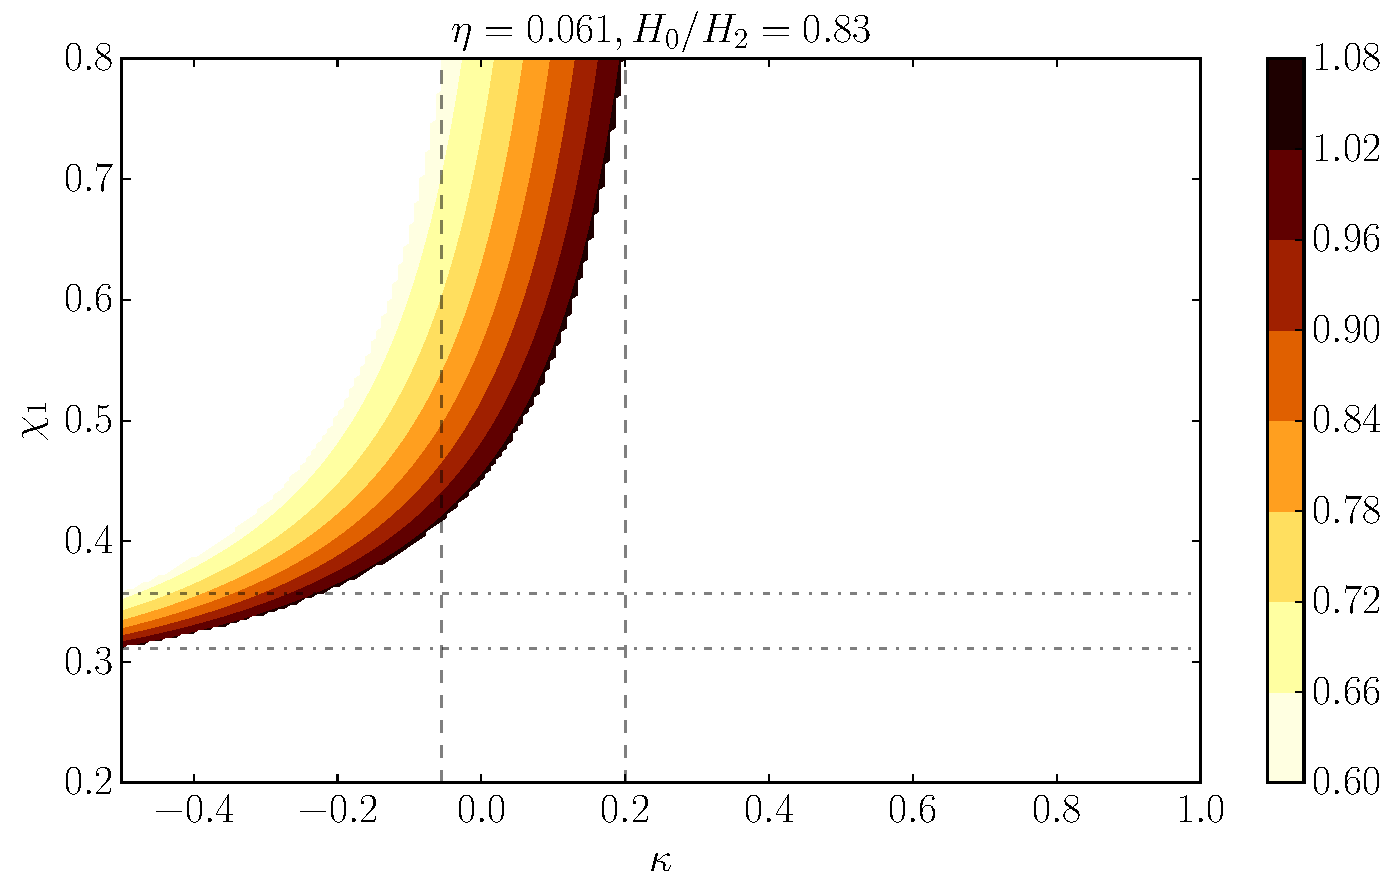
\includegraphics[width=0.8\linewidth]{figures/SM_bounds.pdf} 
\caption{Region of $\chi-\kappa$ parameter space for $\eta=0.06$,
$H_{0}/H_{2}=0.83$, and for $\text{SNR}_2/\text{SNR}_0$  restricted between 0.75
and 1.25. The vertical dashed lines correspond to the upper bound on the value
of $\kappa$ and the spacing between them represents the uncertainty in the
bound, since we've considered a range of SNR ratios close to 1.  Similarly, the
horizontal dotted lines and the spacing between them correponds to the lower bound on
$\chi_{1}$ and it's associated uncertainty respectively.}
\label{chi--kappa_region}
\end{figure}

In Fig.~(\ref{chi--kappa_region})[\textbf{Not complete. Fix text.}]. Further, if we fix the SNR ratio to be equal to 1 (by requiring that both the
SNRs need to be high and comparable to each other for the maximum likelihood
estimation to work), we observe that for a particular value of $\eta$,
$\Sigma(\eta, \chi, \kappa)$ is bounded in the $(\chi, \kappa)$ parameter
space (see Fig.~10\textbf{a}) and the bounds vary over 
$H_{0}/H_{2}$, which in turn, varies from $-1.5$ to $1.5$ over all
combinations of ($\theta_J, \psi_J$). Therefore, by keeping the SNR ratio
constant and varying $H_{0}/H_{2}$ (an effective
orientation parameter that describes the orientation of the
source in the sky), one can determine the bounds on these parameters for a 
specific orientation of the source in the sky.

\begin{figure}[!htbp] \centering
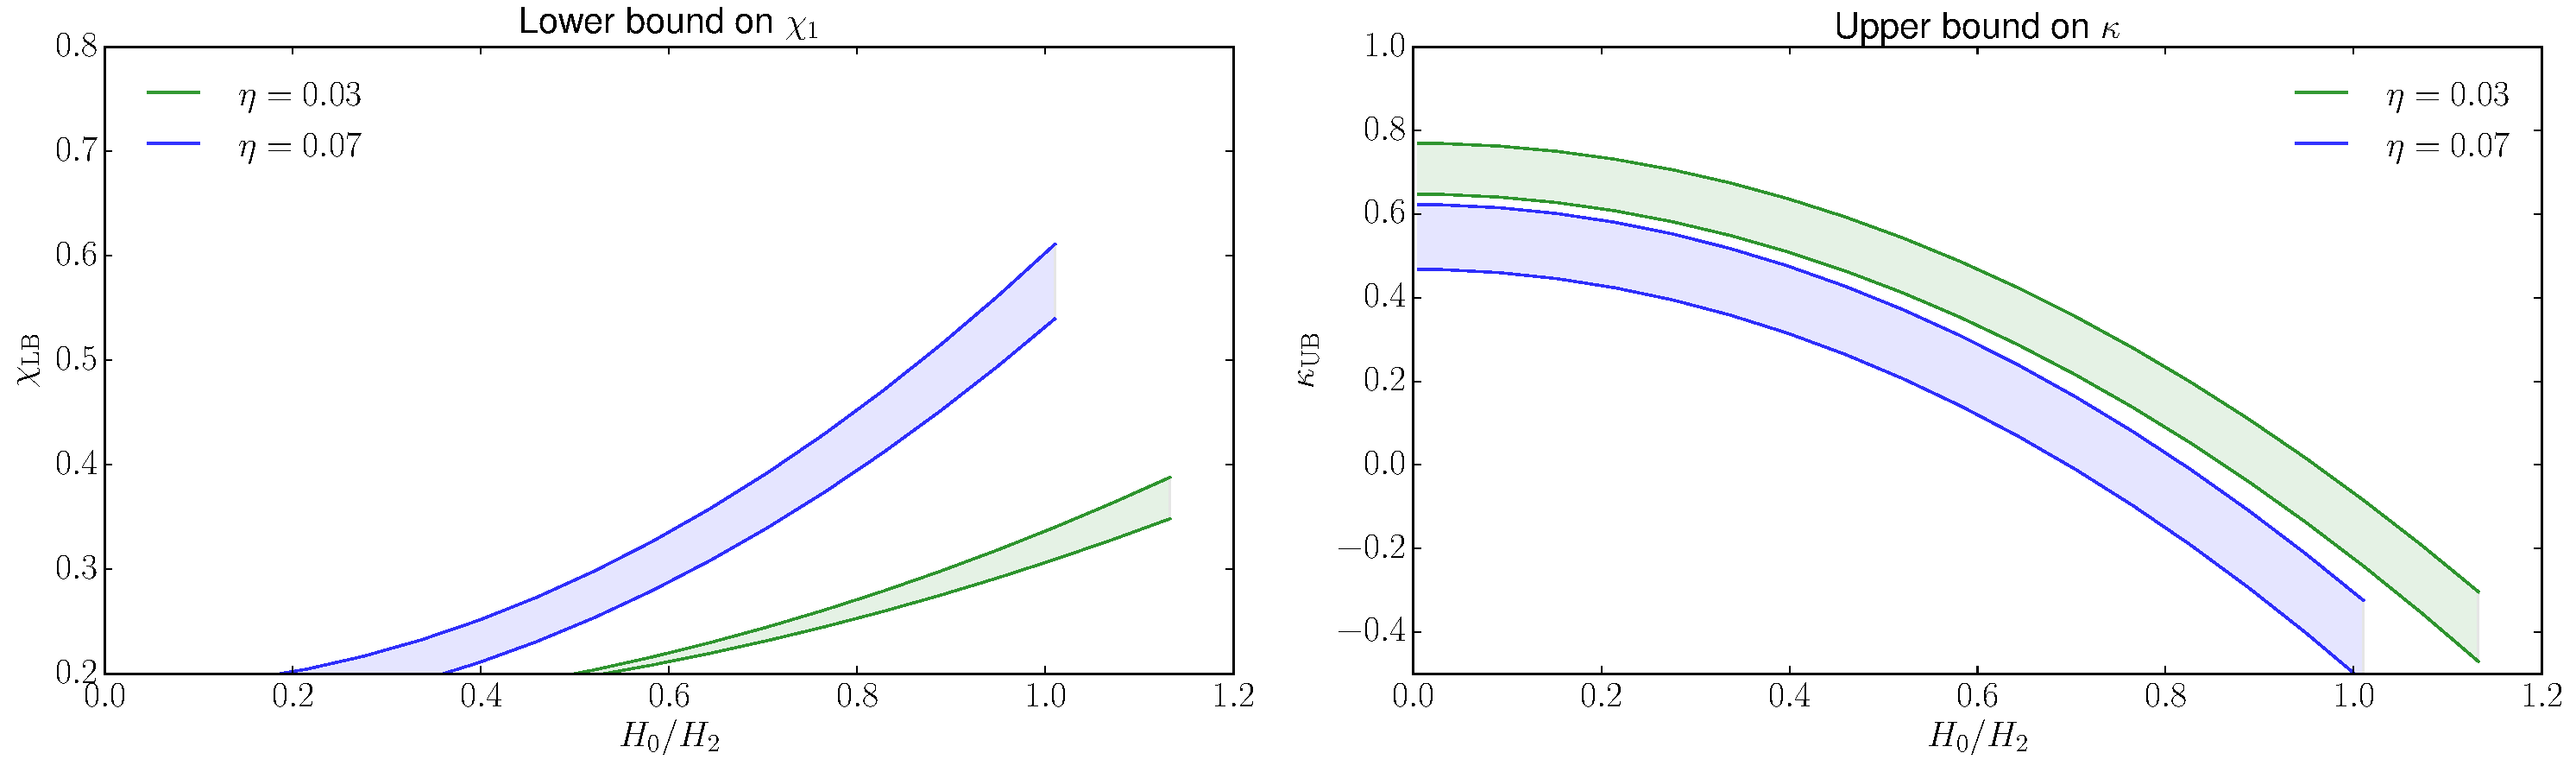
\includegraphics[width=\linewidth]{figures/SM_chi_kappa_bounds.pdf} 
\caption{Bounds}
\label{chi--kappa_bounds}
\end{figure}

In Fig.~(10\textbf{b}) and (10\textbf{c})   we show the variation in the bounds
on $\kappa$ and $\chi$ with respect to $H_{0}/H_{2}$.  The shaded region
corresponds to the uncertainty in the values of upper bound on $\kappa$ in
Fig.~(10\textbf{b}) and the lower bound on $\chi_{1}$ in (10\textbf{c}) if the
SNR ratio is restricted lie between 0.75 and 1.25, i.e.
\begin{equation}
0.75 < \frac{\text{SNR}_{2}}{\text{SNR}_{0}} < 1.25.
\end{equation}
in order to account for the error bar in the estimate of the SNR ratio due to
the presence of detector noise. In both of these figures, the shaded regions
are bounded by parabolae fitted to the data, that are symmetric about
$H_{0}/H_{2} = 0$. We observe that bounds improve (i.e.~the values of the
parameters are better constrained) as the value of $\eta$ increases and the
value of $H_{0}/H_{2}$ is away from $0$. However, the bounds on $\kappa$
and $\chi$ disappear  near $H_{0}/H_{2}=-1.5$ and $H_{0}/H_{2}=1.5$. Further,
the uncertainty in the value of the bounds due to the uncertainty in the SNR
ratio increases with the value of $\eta$, and is minimum when $H_{0}/H_{2}$ is
close to $0$. 

To conclude, we show that it's possible to put one-sided bounds on the
intrinsic parameters (lower bound on $\chi_{1}$ and upper bound $\kappa$) if
we are able to estimate $H_{0}$ and $H_{2}$ and compute their ratio, and to be able do
so, the SNR of each of the individual  sidebands should be high (SM: we need
some estimate here) and comparable to each other. Further, the parameters are better
constrained for systems with comparable masses (i.e. high $\eta$) and for certain orientations
of the source corresponding to values where $H_{0}/H_{2}$ is
away from $0$. (SM: This doesn't really seem to have a physical interpretation, does it?). 
%==============================================================================%
\section{Discussions and conclusion}
\label{conclusion} 
%==============================================================================%
In this work, we studied the contribution of individual harmonics of the single
spin precessing waveform, {\it SpinTaylorF2SingleSpin}. Since, CBC are the most
plausible sources for GW in the sensitivity  range of the modern ground base
interferometric detectors one include the possibility of detecting precessing
compact binaries. In the first observational run of Advance LIGO detectors
precession was not included. However, a NSBH and BBH systems we expect one of
the component(typically the black hole) can posses significant spin which may
lead to a precessing CBC due to which modulation in the waveforms can be
expected.  The analytical waveform model, {\it SpinTaylorF2SingleSpin} is
designed to capture the spin induced precession in a NSBH system.

This work focuses on the overlap study of these individual harmonics with the
full waveform to understand their contribution to the waveform. For our study we
fixed the NS' mass to be $1.4 M_{\odot}$.  We observe that for low BH-spin and
low mass asymmetry(near equal mass systems), ($2,2,2$) modes captures most of
the overlap in the entire parameter space. The same is true for higher mass
asymmetry but  very low BH-spin. Both of these cases refer to non-precessing
systems. Also, for aligned spin cases ($\kappa \simeq 1$) no precession is
expected and we observe that for these regions also ($2,2,2$) is the  dominant
mode. However for high BH-spin and mass asymmetries in certain regions of
parameter space(typically heavily mis-aligned cases) ($2,2,0$) modes seems to
have high overlap values(${\cal{O}}_2 \geq{\cal{O}}_0$).  Typically such regions
have dominant precession effects. Our work focuses on differentiating between
the regions where individual modes or some of the modes has dominant
contribution to the waveform.  Assuming that ($2,2,2$) and ($2,2,0$) are the
only dominant modes we divided the regions of parameter space into three
regions: I- ${\cal{O}}_2 \gg {\cal{O}}_0$, II- ${\cal{O}}_2 \ll() {\cal{O}}_0$
and III- ${\cal{O}}_2$ and ${\cal{O}}_0$ are comparable. We have obtained fits
for these regions in sec.IV. The boundary of the regions obtained by fits are
the function of mass-asymmetry and BH-spin. However,  the region of our
interest, where ${\cal{O}}_2$ and ${\cal{O}}_0$ are comparable should have
significant SNR so that they can be plausible candidate for detection by the
ground based interferometric detector networks.

We also performed a test for our analysis by accumulating points in the three
regions based on the fraction of the total SNR captured by the two dominant
modes  greater than a threshold(typically $.75$). More than $83\%$ of the points
fell into this condition. We also test that out of these points how many points
are actually captured by the fitted regions. The results indicated that more
than $97\%$ of the points in region I and II. For region II more than $4\%$ of
the points are captured into the fitted region. The region for this drop can be
explained by the fact that  we put extra conditions on the individual overlaps
to be greater than $0.4$. However, in this region of parameter space some
contribution to the SNR can come from ($2,2,1$) mode.

The basic motivation for such an analysis comes from the structural form of
these harmonics. The regions, where one of the modes is dominant can be compared
with a fully precessing and non-precessing CBCs. However, for moderately
precessing NSBH systems we need to consider both the harmonics. Filtering the
data with the individual harmonics may give insight about  the angular
distribution of the sources. However, there is a degeneracy over the mass-
asymmetry and spin values in the SNR contribution. If the component masses are
known to a certain accuracy, the BH-spin  can be inferred from the overlap
distribution. Our ongoing work is about extracting these parameters in the
region of interest where these two harmonics have comparable overlaps as well as
contribution to the SNR.



\section{Acknowledgement} 

We thank to K. G. Arun and B. S. Satyaprakash for helpful discussions.  Kumar
Atmjeet and Archana Pai acknowledge the supports from the DST-MPG Max Planck
Partner Group fund at  IISER TVM. \'E Chassande- Mottin acknowledges the support
from CNRS, PICS grant respectively. K. Harris is supported by CSIR-SRF at IISER-
TVM.  This document has a LIGO document number {\bf LIGO-XXXXXXX}.
 
%\includegraphics[width=3.5in]{}
%}
%\label{fit_c_ch}
%\caption{\blue{Comparison of the overlaps of ($2,2,2$) and ($2,2,0$) in the paramter space associated with $OV2<0.6$ for $m_{1}=14M_{\odot}$
% and $\chi_1=0.8$.}}
%\end{figure}

%\begin{figure}
 %\centering
 %{
%\includegraphics[width=5in,height=3.7in,angle=0]
%{C1_for_m_{1}_chi_pt8_after_fit.pdf}
%}
%\label{fit_c_m_{1}}
%\caption{\blue{Comparison of the overlaps of ($2,2,2$) and ($2,2,0$) in the %paramter space associated with $OV2<0.6$ for $m_{1}=14M_{\odot}$
 %and $\chi_1=0.8$.}}
%\end{figure}
\appendix
\section{Precession amplitude functions $z_m$}\label{append}
As described in Sec. \ref{IIb}, $z_m$'s can be expressed in terms of spin-weighted spherical harmonics $\mathstrut_{-2}Y_{2,m}$. Below  we are listing simplified expressions of expressions of $z_m$'s  as functions of $(\theta_J, \psi_J, \beta(f))$.
\begin{eqnarray}
z_2 &=& \cos^4 \frac{\beta}{2}\left[e^{-i2\psi_J}~\cos^4 \frac{\theta_J}{2}+e^{i2\psi_J}~\sin^4 \frac{\theta_J}{2} \right]~,\\
z_1 &=&\sin\frac{\beta}{2}~\cos^3\frac{\beta}{2}~\sin \theta_J \left[e^{-i2\psi_J} (1 +  \cos \theta_J) + e^{i2\psi_J} (1- \cos \theta_J)  \right]  ~,\\
z_0 &=& \frac{3}{4} \sin^2 \beta~\cos2 \psi_J~\sin^2 \theta_J~\\
z_{-1} &=& \cos\frac{\beta}{2}~\sin^3\frac{\beta}{2}~\sin \theta_J \left[e^{-i2\psi_J} (1 -  \cos \theta_J) + e^{i2\psi_J} (1+ \cos \theta_J)  \right]  ~,\\
z_{-2} &=& \sin^4\frac{\beta}{2}~\left[e^{-i2\psi_J} \sin^4\frac{\theta_J}{2} + e^{i2\psi_J} \cos^4\frac{\theta_J}{2} \right] ~.
\end{eqnarray}

\bibliography{STF2}
\end{document}


